\documentclass{article}
\usepackage{ctex}
\usepackage[a4paper,left=10mm,right=10mm,top=15mm,bottom=15mm]{geometry}
\usepackage{graphicx}
\usepackage{amsfonts,amssymb}
\usepackage{amsmath}
\usepackage{biblatex}
\usepackage{hyperref}
\usepackage{color}
\usepackage{titlesec}
\usepackage{titletoc}
\usepackage{listings}

\title{代码大全笔记}
\author{张谦}
\date{\today}
\begin{document}
\maketitle
\tableofcontents
\newpage

\section{欢迎进入软件构件的世界}
\subsection{什么是软件构建}
如下图所示,构建活动主要是编码与调试,但也涉及详细设计、规划构建、单元测试、集成、集成测试
等其他活动。
\begin{figure}[ht]
    \centering
    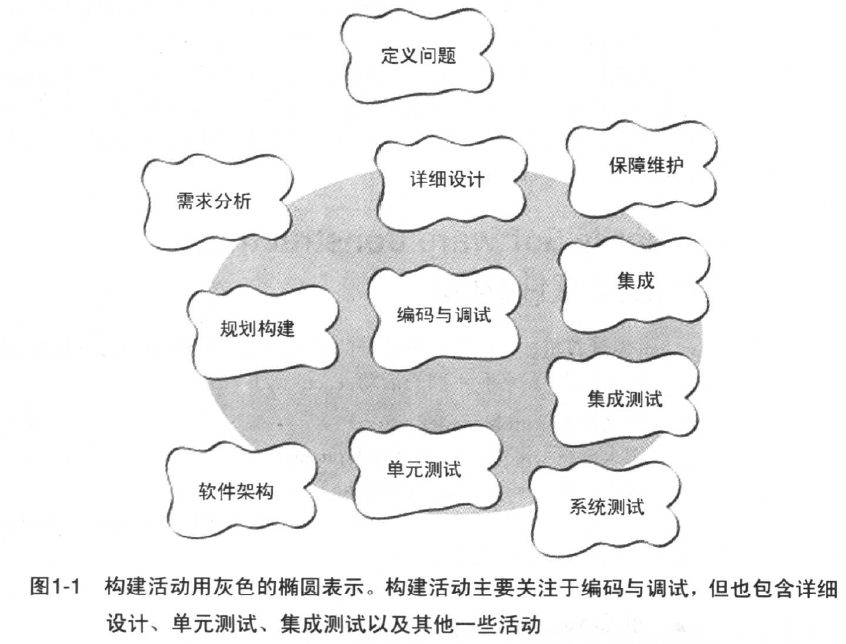
\includegraphics[width=10cm]{figure1.png}
\end{figure}

\par
构建活动包含如下具体任务:
\begin{itemize}
    \item 验证有关的基础工作已经完成,保证构建活动可以顺利进行;
    \item 确定如何测试所写的代码;
    \item 设计并编写类和子程序;
    \item 创建并命名变量和具名常量;
    \item 选择控制结构,组织语句块;
    \item 对代码进行单元测试和集成测试,并排除其中的错误;
    \item 评审开发团队其他成员的底层设计和代码,并让他们评审你的工作;
    \item 优化代码,仔细进行代码的格式化和注释;
    \item 将单独开发的多个组件集成为一体;
    \item 调整代码,让它更快、更省资源。
\end{itemize}

\subsection{构建为什么重要}
\begin{itemize}
    \item 构建活动是软件开发的主要组成部分;
    \item 构建活动是软件开发中的核心活动;
    \item 将主要精力集中于构建活动,可以大大提高程序员生产率;
    \item 构建活动的产物,源代码,往往是对软件的唯一精确描述;
    \item 构建活动是唯一一项确保完成的工作。
\end{itemize}

\section{用隐喻理解软件开发}
隐喻是启示而不是算法,可以将软件开发过程与其他熟悉的活动联系在一起,帮助更好地理解开发过程。
相比其他隐喻,例如写作、种植和养殖等,通过将软件的构建过程,比作房屋的建设过程,能够更好地
理解软件构建的各个阶段。
\subsection{建造隐喻}
\par
(1)问题定义(problem definition):决定准备建一个什么类型的房子;
\par
(2)架构设计(architectural design):和某个建筑师探讨总体设计,并得到批准;
\par
(3)详细设计:画出详细的蓝图,雇一个承包人;
\par
(4)软件构建(construction):准备好建造地点,打好地基,搭建房屋框架,砌好边墙,盖好房顶,
通好水、电、煤气等;
\par
(5)软件优化:在房子大部分完成后,庭院设计师、油漆匠和装修工还要把新盖的房子以及里面的家什
美化一番;
\par
(6)评审和审查(reviews,inspections):在整个过程中,还会有各种监察人员来检查工地、地基、
框架、布线以及其他需要检查的地方。

\subsection{已有组件}
当开发软件时,会大量使用高级语言所提供的功能,而不会自己去编写操作系统层次的代码;
自己编写那些能买得到的现成程序库是没有意义的,例如一些容器类、科学计算函数、用户界面组件、
数据库访问组件等。在建造房子的时候,你也不会去试着建造那些能买得到的东西,例如洗衣机、
冰箱、餐桌等。

\subsection{定制组件}
如果想建造一间拥有一流家具的高档住宅,可能就需要定制的橱柜,以及和橱柜搭配的洗碗机和冰箱等。
在软件开发中也有这种订制的情况,例如想要开发一款一流的软件产品,可能会自己编写科学计算函数,
以便获得更快的速度和更高的精度。

\subsection{防止过度计划}
适当的多层次规划对于建造房屋和构建软件都是有好处的,如果按错误的顺序构建软件,那么编码、测试和
调试都会很难。精心计划,并不是事无巨细的计划或过度计划,例如你可以把房屋的结构性支撑规划清楚,
在日后再决定是用木地板还是瓷砖地板,墙面漆成什么颜色等。

\subsection{不同软件项目}
建筑业中,盖一间仓库或工具房,或是一座医院或核反应站,在规划、设计和质量保证方面所需达到的程度
是不一样的,所用的方法也不相同。同理,在软件开发中,通常只需要用灵活的、轻量级的方法,但有时
你就必须用严格的、重量级的开发方法,以达到所需的安全性目标或其他目标。
另外,还需要特别关注工作时间,在建造帝国大厦时,每辆运料车运输时都留有15分钟的余地,如果
某辆车没能在指定的时间到位,则整个工期就会延误。对于超大型的软件项目,就需要比一般规模的项目
有更高级的规划设计,如果需要创造在经济规模上可以匹敌帝国大厦的庞大软件项目,那么与之相当
水准的技术与管理控制也是必需的。

\section{构建前期准备}
\subsection{前期准备的重要性}
准备工作的中心目标就是降低风险,软件开发中最常见的项目风险是糟糕的需求分析和糟糕的项目计划,
因此准备工作就倾向于集中改进需求分析和项目规划。
高质量的实践方法在项目的初期、中期和末期都强调质量:
\par
(1)如果在项目末期强调质量,那么你会强调系统测试;但是测试只是完整的质量保证策略的一部分,
而且不是最有影响的部分;
\par
(2)如果在项目中期强调质量,那么你会强调构建实践;
\par
(3)如果在项目开始阶段强调质量,那么你就会计划、要求并设计一个高质量的产品;例如你用为吉利车
做的设计来开始整个生产过程,尽管你可以想尽办法来测试,它也绝对不会变成奔驰;也许你能造出最好
的吉利车,但是如果你想要的是奔驰,那么你就得从头开始做设计。

\subsection{序列式开发和迭代式开发选择}
绝大多数的项目都不会完全使用序列式开发法或完全使用迭代式开发法。预先详细说明100\%的需求
和设计是不切实际的,不过对绝大多数项目来说,尽早把那些最关键的需求要素和架构要素确定下来,
时很有价值。
\par
可能因为下列原因选择一个更加迭代的方法:
\begin{itemize}
    \item 需求并没有被理解透彻,或者出于其他理由你认为它是不稳定的;
    \item 设计很复杂,或者有挑战性,或者两者兼具;
    \item 开发团队对于这一应用领域不熟悉;
    \item 项目包含许多风险;
    \item “长期可预测性”不重要;
    \item 后期改变需求、设计和编码的代价很可能比较低。
\end{itemize}
相反的,你可能需要选择一个更加序列的方法。

\subsection{问题定义的先决条件}
在开始构建之前,首先要满足的一项先决条件是,对这个系统要解决的问题做出清楚的陈述。
问题定义只定义了问题是什么,而不涉及任何可能的解决方案。它是一个很简单的陈述,并且听起来
应该像个问题。例如“我们跟不上客户的订单了”听起来就像个问题,而且确实是一个很好的问题
定义;而“我们需要优化数据自动采集系统,使之跟上客户的订单”,这种就是糟糕的问题定义,
它听起来不像问题,而像解决方案。另外,问题定义应该用客户的语言来书写,而且应该从客户的
角度来描述问题。

\subsection{需求的先决条件}
“需求”详细描述软件系统应该做什么,这是达成解决方案的第一步。需求明确有如下好处:
\begin{itemize}
    \item 用户可以自行评审,并进行核准;否则程序员就常常会在编程期间自行决定需求;
    \item 有助于避免争论,如果你和另外一个程序员有分歧,可以查看书面的需求,已解决分歧;
    \item 有助于减少开始编程开发之后的系统变更的情况;
    \item 充分详尽地描述需求,是项目成功的关键,它甚至很可能比有效的构建技术更重要。
\end{itemize}

\par
在构建期间处理需求变更,有以下一些可以采用的方式:
\begin{itemize}
    \item 评估需求质量,如果需求不够好,则停止工作,退回去,先做好后再继续前进;
    \item 确保每一个人都知道需求变更的代价;
    \item 建立一套变更控制程序;
    \item 使用能适应变更的开发方法;
    \item 放弃这个项目;
    \item 注意项目的商业案例,注重商业价值。
\end{itemize}

\subsection{架构的先决条件}
软件架构是软件设计的高层部分,是用于支持更细节设计的框架。架构的质量决定了系统的“概念完整性”,
继而决定了系统的最终质量。一个经过慎重考虑的架构,为“从顶层到底层维护系统的概念完整性”,提供
了必备的结构和体系,它为程序员提供了指引,其细节程度与程序员的技能和手边的工作相配;它将
工作分为几个部分,使多个开发者或多个开发团队可以独立工作。
\par
架构的典型组成部分:
\par
(1)程序组织:
\begin{itemize}
    \item 系统架构首先要以概括的形式对有关系统做一个综述;
    \item 在架构中,应该能发现对那些曾经考虑过的,最终组织结构的,替代方案的记叙;
    找到之所以选用最终的组织结构,而不是其他替代方案的理由;
    \item 架构应该定义程序的主要构造块,根据程序规模的不同,各个构造块可能是单个类,也可能是由
    许多类组成的一个子系统;
    \item 应该明确定义各个构造块的责任,每个构造块应该负责某一个区域的事情,并且对其他构造块负责的
区域知道得越少越好,将设计的信息局限在各个构造块之内;
    \item 应该明确定义每个构造块的通信规则,对于每个构造块,架构应该描述它能直接使用那些构造块,能
间接使用哪些构造块,不能使用哪些构造块。
\end{itemize}

\par
(2)主要的类:
\begin{itemize}
    \item 架构应该详细定义所用的主要的类,应该指出每个主要的类的责任,以及该类如何与其他类交互;
    它应该包含对类的继承体系、状态转换、对象持久化等的描述;如果系统足够大,它应该描述如何将
    这类组织成一个个子系统;
    \item 架构应该记述曾经考虑过的其他类设计方案,并给出选用当前方案的理由;架构无需详细说明
    系统中的每一个类,利用80/20法则:对那些构成系统80\%的行为的20\%的类进行详细说明。
\end{itemize}

\par
(3)数据设计:
\begin{itemize}
    \item 架构应该描述所用到的主要文件和数据表的设计。它应该描述曾经考虑过的其他方案,并说明
    选择当前方案的原因。如果应用程序要维护一个客户ID的列表,而架构师决定使用顺序访问的列表来
    表示该ID的列表,那么文档就应该解释为什么顺序访问的列表比随机访问的列表、堆栈、散列表要好。
    在构建期间,这些信息让你能洞察架构师的思想;在维护阶段,这种洞察力是无价之宝。离开它,你就像
    看一部没有字幕的外语片;
    \item 数据通常只应该由一个子系统或一个类直接访问;例外的情况就是通过访问器类或访问器子程序,
    以受控且抽象的方式来访问数据;
    \item 架构应该详细定义所用数据库的高层组织结构和内容;架构应该解释为什么单个数据库比多个数据库
    要好,反之亦然。需要解释为什么不用平坦的文件,而要用数据库,指出与其他访问同一数据的程序的
    可能交互方式,说明创建哪些数据视图等等。
\end{itemize}

\par
(4)业务规则:
\par
如果架构依赖于特定的业务规则,那么它就应该详细描述这些规则,并描述这些规则对系统设计的影响。例如,
假定要求系统遵循这样一条业务规则:客户信息过时的时间不能超过30秒。在此种情况下,架构就应该描述
这条规则对架构采用的“保持客户信息及时更新且同步”的方法的影响。

\par
(5)用户界面设计:
\par
\begin{itemize}
    \item 用户界面常常在需求阶段进行详细说明,如果没有,就应该在软件架构中进行详细说明。架构
    应该详细定义Web页面格式、GUI、命令行接口等主要元素;
    \item 架构应该模块化,以便在替换为新用户界面时,不影响业务规则和程序的输出部分。例如,架构应该
    使我们很容易做到:砍掉交互式界面的类,插入一组命令行的类。这种替换能力常常很有用,由其
    因为命令行界面便于单元级别和子系统级别的软件测试。1
\end{itemize}

(6)资源管理:
\par
架构应该描述一份管理稀缺资源的计划。稀缺资源包括数据连接、线程、句柄等。在内存受限的应用领域,如
驱动程序开发和嵌入式系统中,内存管理是架构应该认真对待的另一个重要领域。架构应该应该估算在正常情况和
极端情况下的资源使用量。在简单的情况下,估算数据应该说明:预期的运行环境有能力提供所需的资源,
在更复杂的情况下,也许会要求应用程序更主动地管理其拥有的资源。如果是这样,那么资源管理器应该和
系统的其他部分一样,进行认真的架构设计。

\par
(7)安全性:
\par
架构应该描述实现设计层面和代码层面的安全性的方法。如果先前尚未建立威胁模型,那么就应该在架构阶段
建立威胁模型。在制定编码规范的时候,应该把安全性牢记在心,包括处理缓冲区的方法、处理非受信数据
(用户输入数据、cookies、配置数据和其他外部接口输入的数据)的规则、加密、错误信息的细致程度、
保护内存中的秘密数据,以及其他事项。

\par
(8)性能:
\par
如果需要关注性能,就应该在需求中详细定义性能目标。性能目标可以包括资源的使用,这时,性能目标也应该
详细定义资源(速度、内存、成本)之间的优先顺序。架构应该提供估计的数据,并解释为什么架构师相信能
达到性能目标。如果某些部分存在达不到性能目标的风险,那么架构也应该指出来。如果为了满足性能目标,
需要在某些部分使用特定的算法或数据类型,架构应该说清楚。架构中也可以包括各个类或各个对象的
空间和时间预算。

\par
(9)可伸缩性:
\par
可伸缩性是指系统增长以满足未来需求的能力。架构应该描述系统如何应对用户数量、服务器数量、网络节点数量、
数据库记录数、数据库记录的长度、交易量等的增长。如果预计系统不会增长,而且可伸缩性不是问题,
那么架构应该明确地列出这一假设。

\par
(10)互用性:
\par
如果预计这个系统会与其他软件或硬件共享数据或资源,架构应该描述如何完成这一任务。

\par
(11)国际化和本地化:
\par
国际化是一项准备让程序支持多个地域的技术活动。国际化常常称为“I18n",因为国际化的英文单词
“Internationalization”首尾两个字符之间有18个字母。本地化活动是翻译一个程序,以支持当地特定的
语言工作。

\par
(12)输入输出:
\par
输入输出(I/O)是架构中值得注意的另一个领域。架构应该详细定义读取策略是先做、后做还是即时做。
而且应该描述在哪一层检测I/O错误:在字段、记录、流,或者文件的层次。

\par
(13)错误处理:
\par
错误处理已被证实为现代计算机科学中最棘手的问题之一,不能武断地处理它。因为错误处理牵连到整个系统,
因此最好在架构层次上对待它:
\begin{itemize}
    \item 错误处理是进行纠正还是仅仅进行检测?如果是纠正,程序可以尝试从错误中恢复过来。如果
    仅仅是检测,那么程序可以像没发生任何事一样继续运行,也wiagua可以退出。无论哪种情况,都应该通知
    用户说检测到一个错误;
    \item 错误检测时主动的还是被动的?系统可以主动地预测错误,例如,通过检查用户输入的有效性,也
    可以在不能避免错误的时候,被动地响应错误,例如,当用户输入的组合产生了一个数值溢出错误时。
    前者可以扫清障碍,后者可以清除混乱。同样,无论采用哪种方案,都与用户界面有影响;
    \item 程序如何传播错误?程序一旦检测到错误,它可以立刻丢弃引发错误的数据;也可以把这个错误当成
    一个错误,并进入错误处理状态;或者可以等到所有处理完成,再通知用户说在某个地方发现了错误;
    \item 错误消息的处理有什么约定?如果架构没有详细定义一个一致的处理策略,那么用户界面看起来
    就像“令人困惑的乱七八糟的抽象拼贴画”,由程序的不同部分的各种界面拼接而成。要避免这种外观体验,
    架构应该建立一套有关错误消息的约定;
    \item 如何处理异常?架构应该规定代码何时能够抛出异常,在什么地方捕获异常,如何记录这些异常,以及
    如何在文档中描述异常等等;
    \item 在程序中,在什么层次上处理错误?你可以在发现错误的地方处理,可以将错误传递到专门处理
    错误的类进行处理,或者沿着函数调用链往上传递错误;
    \item 每个类在验证其输入数据的有效性方面需要负何种责任?是每个类负责验证自己的数据有效性,
    还是有一组类负责验证整个系统的数据的有效性?某个层次上的类是否能假设它接收的数据是干净的?
    \item 你是希望用运行环境中内建的错误处理机制,还是想建立自己的一套机制?事实上,运行环境
    所拥有的某种特定的错误处理方法,并不是符合你需求的最佳方法。
\end{itemize}

\par
(14)容错性:
\par
架构还应该详细定义所期望的容错种类。容错是增强系统可靠性的一组技术,包括检测错误:如果可能的话,
从错误中回复;如果不能从错误中回复,则包容其不利影响。例如,为了计算某数的平方根,系统的容错
策略有以下几种:
\begin{itemize}
    \item 系统在检测到错误的时候退回去,再试一次。如果第一次的结果是错误的,那么系统可以退回
    到之前一切正常的时刻,然后从该点继续运行;
    \item 系统拥有一套辅助代码,以备在主代码出错时使用。在本例中,如果发现第一次的答案似乎错误,
    系统就切换到另一个计算平方根的子程序,以取而代之;
    \item 系统使用一种表决算法。它可以有三个计算平方根的类,每一个都使用不同的计算方法;
    每个类分别计算平方根,然后系统对结果进行比较;根据系统内建的容错机制的种类,系统可以以
    三个结果的均值、中值或众数作为最终结果;
    \item 系统使用某个不会对系统其余部分产生危害的虚假值代替这个错误的值;
    \item 其他容错方法包括,在遇到错误时,让系统转入某种部分运转状态,或者转入某种功能退化状态;
    系统可以自动关闭或重启。
\end{itemize}

\par
(15)架构的可行性:
\par
设计师关注系统的各种能力,例如是否能达到性能目标,能够在有限的资源下运转,运行环境是否有足够的
支持。架构应该论证系统的技术可行性。如果在任何一个方面不可行,都会导致项目无法实施;那么架构
应该说明“这些问题是如何经过研究的”,通过验证概念的原型、研究或其他手段,必须在全面开展构建之前
解决掉这些风险。

\par
(16)过度工程:
\par
健壮性(robustness)是指系统在检测到错误后,继续运行的能力。通常架构详细描述的系统,会比需求详细
描述的系统更健壮。理由之一为,如果组成系统的各个部分都只能在最低限度上,满足健壮性要求,那么
系统整体上是达不到所有要求的健壮程度的。在软件中,链条的强度不是取决于最薄弱的一环,而是等于所有
薄弱环节的乘积。架构应该清楚地指出程序员应该“为了谨慎起见,宁可进行过度工程(overengineering)”,
还是应该做出最简单的能工作的东西。
\par
详细定义一种过度工程的方法尤其重要,因为许多程序员会出于专业自豪感,对自己编写的类做过度工程。通过
在架构中明确地设立期望目标,就能避免出现“某些类异常健壮,而其他类勉强够健壮”的现象。

\par
(17)关于“买”还是“造”的决策:
\par
如果架构不采用现货供应的组件,那么就应该说明“自己定制的组件,应该在哪些方面胜过现成的程序库和组件”。

\par
(18)关于复用的决策:
\par
如果开发计划提倡使用业已存在的软件、测试用例、数据格式或其他原料,架构应该说明:如何对复用的软件
进行加工,使之符合其他架构目标(如果需要使之符合的话)。

\par
(19)变更策略:
\par
面对变更,软件架构师面临的一个主要挑战,是让架构足够灵活,能够适应可能出现的变化。
\begin{itemize}
    \item 架构应当清楚地描述处理变更的策略。架构应该列出已经考虑过的可能会有所增强的功能,并说明
    “最有可能增强的功能,同样也是最容易实现的”。如果变更很可能出现在输入输出格式、用户交互的风格、
    需求的处理等方面,那么架构就应该说明:这些变更已经被预料到了,并且任何单一的变更都只会影响
    少数几个类。架构应该对变更的计划可以很简单,比如在数据文件中放入版本号、保留一些供将来使用的
    字段、或者将文件设计成能够添加新的表格。如果使用了代码生成器,那么架构应该说明,可预见的变更
    都不会超出该代码生成器的能力范围;
    \item 架构应该指出“延迟提交”所用的策略。比如说,架构也许规定使用表驱动技术。它也许还规定
    “表”中的数据是保存在外部文件中,而非直接写在代码中,这样就能做到在不重新编译的情况下修改程序。
\end{itemize}

\par
(20)架构的总体质量:
\par
优秀的架构规格书的特点在于,讨论了系统中的类、讨论了每个类背后的隐藏信息、讨论了“采纳或排斥
所有可能的设计替代方案”的根本理由。
\begin{itemize}
    \item 架构应该是带有少许特别附加物的,精炼且完整的概念体系。好的架构设计,应该与待解决的
    问题和谐一致;
    \item 在架构开发过程中的多种变更方式,每一项变更,都应该干净地融入整体概念;
    \item 架构的目标应该清楚地表述;
    \item 架构应该描述所有主要决策的动机;
    \item 优秀的软件架构,很大程度上是与机器和编程语言无关的;要尽可能地独立于环境;如果程序
    的用途就是去试验某种特定的机器或语言,那么这条指导原则就不适用了;
    \item 架构应该处于对系统,“欠描述”和“过度描述”之间的那条分界线上;设计者不应该将注意力放在
    某个部件上,而损害其他部件;
    \item 架构应该明确地指出有风险的区域;它应该解释为什么这些区域是有风险的,并说明已经采取了
    哪些步骤以使风险最小化;
    \item 架构应该包含多个视角,包括暴露隐藏的错误和不一致的情况,以及帮助程序员完整地理解系统的设计;
    \item 最后,架构不应该包含任何对你而言,很难理解的东西。
\end{itemize}

\subsection{花费在前期准备上的时间}
花费在问题定义、需求分析、软件架构上的时间,依据项目的需要而变化。一般说来,一个运作良好的项目,
会在需求、架构以及其他前期计划方面,投入$10\%-20\%$的工作量,和$20\%-30\%$的时间。这些时间
不包括详细设计的时间,因为详细设计是构建活动的一部分。


\section{关键的构建决策}
\subsection{选择编程语言}
研究表明,编程语言的选择从多个方面,影响生产率和代码质量。程序员使用熟悉的语言时,生产率比使用
不熟悉的语言时要高。使用高级语言的程序员,能比使用较低级语言的程序员,达到更好的生产率和质量。
每种编程语言都有其优点和弱点,要知道你使用的语言的明确优点和弱点。

\subsection{编程约定}
在高质量的软件中,可以看到“架构的概念完整性”,与“底层实现”之间的关系。“实现”必须与指导该实现的
“架构”保持一致,并且这种一致性是内在的、固有的。这正是变量名称、类的名称、子程序名称、格式约定、
注释约定等这些针对“构建活动”的指导方针的关键所在。在“构建”开始之前,讲清楚你使用的编程约定,
编码约定的细节,要达到这样的精确度:在编写完软件之后,几乎不可能改变软件所遵循的编码约定。

\subsection{深入一种语言去编程}
需要理解“在一种语言上编程”和“深入一种语言去编程”的区别。大多数重要的编程原则,并不依赖于特定的
语言,而依赖于你使用语言的方式。如果你使用的语言缺乏你希望的构件,或者倾向于出现其他种类的问题,
那就应该试着去弥补它,发明你自己的编码约定、标准、类库以及其他改进措施。

\section{软件构建中的设计}
软件设计是指构思、创造或发明一套方案,把一份计算机软件的规格说明书要求,转变为可实际运行的软件。
设计就是把需求分析和编码调试连接在一起的活动。好的高层设计能提供一个可以稳妥容纳多个较低层次设计
的结构。
\subsection{设计中的挑战}
(1)设计是一个Wicked问题:
\par
Wicked问题是指那种只能通过解决或部分解决才能被明确的问题。你必须首先把这个问题“解决”一遍,
以便能够明确地定义它,然后再次解决该问题,从而形成一个可行的方案。例子,有一座桥,设计时主要
考虑的问题为是否足够结实,以承受设计负荷;没有意识到大风带来的横向谐波,最终导致大桥坍塌。

\par
(2)设计是一个了无章法的过程:
\par
软件设计的成果应该是组织良好、干净利落的,然而形成这个设计的过程,却并非如此清爽。
\begin{itemize}
    \item 在设计过程中你会采取很多错误的步骤,多次误入歧途。事实上,犯错正是设计的关键所在,
    在设计阶段犯错并加以改正,其代价要比在编码后才发现同样的错误,并彻底修改低得多;
    \item 优劣设计之间的差异,往往非常微妙;
    \item 很难判断设计何时算是“足够好”了。
\end{itemize}

\par
(3)设计是确定取舍和调整顺序的过程:
\par
设计的一个关键内容,是去衡量彼此冲突的各项设计特性,例如存储空间、占用的网络带宽、时间成本等。

\par
(4)设计涉及到诸多限制
\par
设计的要点,一部分是在创造可能发生的事情,而另外一部分又是在限制可能发生的事情。如果人们在建造房屋时,
拥有无限的时间、资源和空间,那么你会看到房屋不可思议地随意蔓延,每幢楼都有上百间屋子,一只鞋
就可以占用一间屋子。

\par
(5)设计是不确定的:
\par
如果让三个人去设计一套同样的程序,可能会有三套截然不同的设计。

\par
(6)设计是一个启发式过程:
\par
因为设计充满了不确定性,因此设计也就趋于具有探索性,而不是保证能产生预期结果的课重复过程,
设计过程中总会有试验和犯错误。

\par
(7)设计是自然而然形成的:
\par
设计是在不断地设计评估、非正式讨论、写试验代码以及修改试验代码中演化和完善的。

\subsection{关键的设计概念}
好的设计源于对一小批关键设计概念的理解。这一节将会讨论:复杂度所扮演的角色、设计应具有的特征、
以及设计层次。
\par
(1)复杂度管理:
\par
\begin{itemize}
    \item 本质问题和偶然问题:本质属性是一件事物必须具备、如果不具备就不再是该事物的属性;
    例如,汽车必须具有发动机、轮子和车门,否则就不能称其为汽车。偶然属性是指一件事物恰巧具有
    的属性,有没有这些属性,并不影响这件事物本身;例如,一辆汽车可能有不同的发动机,但是
    都是一辆汽车。软件开发中,大部分的偶然性难题,很久以前就得到解决了,例如,由笨拙的语法相关
    的偶然问题,大多已经从汇编语言到第三代编程语言的演进过程中解决了;集成编程环境更是进一步解决
    了由于开发工具之间,无法很好地协作而带来的效率问题。软件开发剩下的那些本质性难题,将会变得
    相对缓慢;究其原因,是因为从本质上说,软件开发就是不断地去发掘错综复杂、相互连接的整套
    概念的所有细节。即使我们能发明出一种与现实中,亟待解决的问题,有着相同术语的编程语言,但是
    人们想清楚地认清现实世界到底如何运作,仍然有很多挑战,因此编程仍会十分困难。当软件要解决更大
    规模的现实问题时,现实的实体之间的交互行为,就变得更为复杂,这些转而又增加软件解决方案的本质性
    问题。所有这些本质性困难的根源,都在于复杂性,不论是本质的,还是偶然的;
    \item 管理复杂度的重要性:在对导致软件项目失败的原因进行调查时,人们很少把技术原因归为项目
    失败的首要因素。项目的失败,大多数都是由于差强人意的需求、规划和管理所导致的。但是,当项目
    由技术因素导致失败时,其原因通常就是失控的复杂度。当没人知道对一处代码的改动,会对其他代码
    带来什么影响时,项目也就块停止进展了。因此管理负责度,是软件开发中最为重要的技术话题。
    \item 如何应对复杂度:
    作为软件开发人员,我们不应该试着在同一时间,把整个程序都塞进自己的大脑,而应该试着以某种方式去组织
    程序,以便能够在一个时刻,可以专注于一个特定的部分。这么做的目的是尽量减少在任一时间段内,
    所要考虑的程序量。在软件架构的层次上,可以通过把整个系统分解为多个子系统,来降低问题的复杂度。
    人类更容易理解许多项简单的信息,而不是一项复杂的信息。所有软件设计技术的目标,都是把复杂问题
    分解为简单的部分。子系统的相互依赖越少,你就越容易在同一时间里,专注问题的一小部分。精心设计
    的对象关系,使关注点相互分离,从而使你能在每个时刻,只关注一件事情。保持子程序(函数)的
    短小精悍,也能帮助你减少思考的负担。高代价、低效率的设计源于下面三种根源:
    \begin{itemize}
        \item 用复杂的方法,解决简单的问题;
        \item 用简单但错误的方法,解决复杂的问题;
        \item 用不恰当的复杂方法,解决复杂的问题。
    \end{itemize}
    现代的软件本身就很复杂,无论你多努力,最终都会与存于现实世界问题本身的,某种程度的复杂性不期而遇。
    这就意味着要用下面这两种方法来管理复杂度:
    \begin{itemize}
        \item 把任何人在同一时间,需要处理的本质复杂度的量,减到最少;
        \item 不要让偶然的复杂度无谓地快速增长。
    \end{itemize}
    一旦你能理解软件开发中,任何其他技术目标,都不如管理复杂度重要时,众多设计上的考虑,就都
    变得直截了当了。
\end{itemize}

\par
(2)良好的设计特征:
\begin{itemize}
    \item 最小的复杂度:应该做简单且易于理解的设计,如果你的设计方案,不能让你在专注于程序的
    一部分时,安心地忽视其他部分,这一设计就没有什么作用了;
    \item 易于维护:请时刻想着维护程序员,可能对你的代码提出的问题,把维护程序员当成你的听众,
    进而设计出能自明的系统来;
    \item 松散耦合:在设计时,让程序的各个组成部分之间,关联最小。通过应用类接口中的合理抽象、
    封装性以信息隐藏等原则,设计出相互关联尽可能最少的类。减少关联也就减少了集成、测试与维护时
    的工作量;
    \item 可扩展性:能增强系统的功能,而无须破坏其底层结构。你可以改动系统的某一部分,而不会影响其他
    部分;
    \item 可重用性:所这几的系统的组成部分,能在其他系统中重复利用;
    \item 高扇入:让大量的类,使用某个给定的类;设计出的系统很好地利用了,在较低层次上的工具类;
    \item 低扇出:让一个类里,少量或适中使用其他的类;高扇出(超过约7个),说明一个类使用了
    大量其他的类,因此可能变得过于复杂;
    \item 可移植性:能方便移植到其他环境中;
    \item 精简性:设计出的系统没有多余部分;伏尔泰曾说,一本书的完成,不在它不能再加入任何内容
    的时候,而在不能再删去任何内容的时候。任何多余的代码,需要开发、复审和测试,并且当修改了其他
    代码之后,还要重新考虑它们;
    \item 层次性:尽量保持系统各个分解层的层次性,使你能在任意的层面上观察系统,并且得到某种具有
    一致性的看法,设计出来的系统应该能在任意层次上观察,而不需要进入其他层次;
    例如,假设你在编写一个新系统,其中用到很多设计不佳的旧代码,这是你就应该为新系统编写一个,
    负责同旧代码交互的层。层次化设计的溢出有:(a)将低劣代码的烂泥潭禁闭起来;(b)如果你最终能
    抛弃或重构旧代码,那是就不必修改除交互层之外的任何新代码;
    \item 标准技术:一个系统所依赖的外来的、古怪的东西越多,别人在第一次想要理解它的时候就越是头疼;
    要尽量用标准化的、常用的方法,让整个系统给人一种熟悉的感觉。
\end{itemize}

\par
(3)设计层次:
\par
如下图所示,一个软件系统包含有多个设计层次。
\begin{figure}[ht]
    \centering
    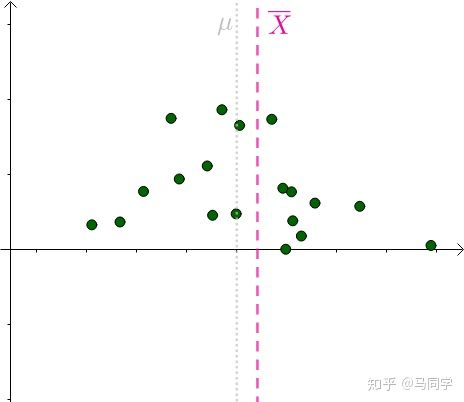
\includegraphics[width=15cm]{figure2.png}
\end{figure}
\begin{itemize}
    \item 第1层:软件系统。第一个层次就是整个系统,需要分解为子系统或包。
    \item 第2层:子系统或包。这一层的主要设计活动,就是确定如何把整个系统分为主要的子系统,并且定义
    清楚允许各子系统,如何使用其他子系统。这些子系统可能会很大,比如数据库、用户界面、业务规则、
    命令解释器、报表引擎等。在这一层的设计中,子系统之间的相互通信规则特别重要。如果所有的子系统
    都能和其他子系统通信,就完全失去了把它们分开所带来的好处。因此,应该通过限制子系统之间的
    通信,来让每个子系统更有存在的意义。
    \par
    例如,如下图所示,假设将系统分为6个子系统。在没有定义任何规则时,热力学第二定律就会发生作用,
    整个系统将会熵增。熵增的一种原因是,如果不对子系统间的通信加以任何限制,那么它们之间的通信就会
    肆意发生。
    \begin{figure}[ht]
        \centering
        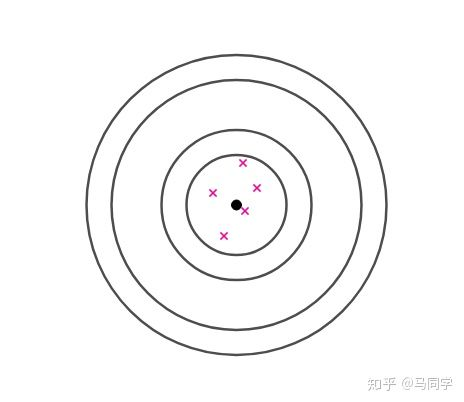
\includegraphics[width=10cm]{figure3.png}
    \end{figure}
    这里的每个子系统,最终都会直接与所有其他子系统进行通信,如果改动某一个子系统,则其他所有和其
    通信的子系统,都需要修改,这样是不合理的。因此需要限制子系统之间的通信,如下图所示,为施加了
    少量通信规则后的系统,
    \begin{figure}[ht]
        \centering
        
\includegraphics[width=10cm]{figure4.png}
    \end{figure}
    另外,为了让子系统之间的连接简单、易懂、且易于维护,就要尽量简化子系统之间的交互关系。最简单
    的交互关系,是让一个子系统,去调用另一个子系统中的子程序;稍微复杂一点的交互,是在一个子系统
    中,包含另一个子系统中的类;而最复杂的交互关系,是让一个子系统中的类,继承另一个子系统中的类。
    \par
    设计子系统,有一条很好的基本原则,即系统层设计图,应该是无环图;亦即程序中不应该有任何环形关系,
    比如说A类使用了B类、B类使用了C类、而C类又实用了A类这种情况。
    \par
    有些种类的子系统,会在不同的系统中反复出现,例如:
    \begin{itemize}
        \item 业务规则:指那些在计算机系统中,编入的法律、规则、政策以及过程;
        \item 用户界面:应创建一个子系统,把用户界面组件,同其他部分分隔开,以便用户界面的演化
        不会破坏程序的其余部分;在大多数情况下,用户界面子系统会使用多个附属的子系统或类,来处理
        用户界面、命令行接口、菜单操作、窗体管理、帮助系统等等;
        \item 数据库访问:可以将对数据库访问的实现细节隐藏起来,让程序的绝大部分,可以不必关心处理
        底层结构的繁琐细节,并能像在业务层次一样处理数据;
        \item 对系统的依赖性:把对操作系统的依赖因素,归到一个子系统里,就如同把对硬件的依赖因素,封装
        起来一样。例如,开发的程序不仅能在windows上运行,也应该可以方便地移植到linux或Mac OS上,
        且只需要修改接口子系统就可以了。
    \end{itemize}
    \item 第3层:分解为类。这一层的主要设计任务,是把所有的子系统,进行适当的分解,并确保分解出的
    细节都恰到好处,能够用单个的类实现。当定义子系统中的类时,也就同时定义了这些类与系统其余部分打交道
    的细节,尤其是要确定好类的接口。例如,数据库子系统可能会被进一步划分成数据库访问类、持久优化
    框架类、以及数据库元数据。
    \par
    类与对象的比较:面向对象设计的一个核心概念,就是对象(object)与类(class)的区分。对象是指运行
    期间,在程序中实际存在的具体实体,而类是指在程序源码中,存在的静态事物。对象是动态的,它拥有
    你在程序运行期间所能得到的具体的值和属性。例如,你可以定义一个名为Person的类,它具有姓名、
    年龄、性别等属性,在程序运行期间,你可以有nancy、hank、tony等对象,它们是类的具体实例。
    \item 第4层:分解成子程序。这一层的设计,包括把每个类细分为子程序(函数)。在第3层中,定义出
    类的接口,已经定义了其中一些子程序,而该层的设计,将细化出类的其他子程序。当你查看类里面
    子程序的细节时,就会发现很多子程序都很简单,但也有些子程序,是由更多层次的子程序所组成,这就
    需要更多的设计工作了。这一层次的分解和设计,通常是留给程序员个人来完成的。
    \item 第5层:子程序内部的设计。这里的设计工作,包括编写伪代码、选择算法、组织子程序内部的
    代码块,以及用何种编程语言编写代码。
\end{itemize}

\subsection{启发式设计方法}
由于软件设计是非确定性的,因此,灵活熟练地运用一组有效的启发式方法,便成了合理的软件设计核心工作。
\par
(1)找出现实世界中的对象:
\par
在确定设计方案时,首选且最流行的是面向对象的设计方法。此方法的要点是辨明现实世界中的对象,以及
人造的对象。使用对象设计的步骤:
\begin{itemize}
    \item 辨识对象及其属性:计算机程序通常都是基于现实世界的实体。例如,如下图所示,可以基于
    现实世界中的雇员(Employee)、顾客(Client)、工作时间记录(Timecard)、以及账单(Bill)等实体,
    来开发一套按时间计费的系统;
    \begin{figure}[ht]
        \centering
        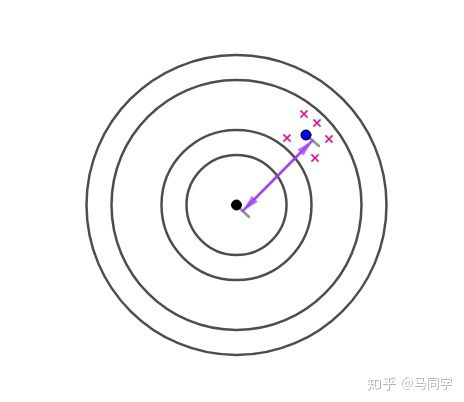
\includegraphics[width=10cm]{figure5.png}
    \end{figure}
    辨识对象的属性,并不比辨识对象本身更困难。每个对象都有一些与计算机程序相关的特征。例如,在这个
    收费系统里,每个雇员对象都具有名字(name)、职务(title)和费率(billingRate)等属性;而顾客对象
    则具有名字(name)、账单寄送地址(billingAddress)、以及账户余额(accountBalance)的属性;账单
    对象具有收费金额、顾客名字、支付日期(billDate)等等。
    \item 确定可以对各个对象进行的操作:在每个对象上,都可以执行多种操作;例如,雇员对象可能需要
    修改职务或者费率,顾客对象可能需要修改名字,或者账单寄送地址等等;
    \item 确定各个对象能对其他对象进行的操作:对象之间最常见的两种关系是包含和继承;一个Timecard
    对象可以包含一个Employee对象和一个Client对象,一个Bill对象可以包含一个或多个Timecard对象;
    另外,一份账单可以标示是否已经给某位顾客开过账单了,而顾客也可以签付一份账单;
    \item 确定对象的哪些部分,对其他对象可见:哪些部分是public的,哪些是private的;
    \item 定义每个对象的public接口:在编程语言的层次上,为每个对象定义具有正式语法的接口。对象对
    其他对象暴露的数据及方法,都被称为该对象的“public接口”,而对象通过继承关系,向其派生
    对象暴露的部分,则被称为“protected接口”。
\end{itemize}
经过上述这些步骤得到一个高层次的、面向对象的系统组织结构之后,你可以用这两种方法来迭代:在高层次的
系统组织结构上进行迭代,以便更好地组织类的结构;或者在每个已经定义好的类上进行迭代,把每个类的设计
详细化。

\par
(2)形成一致的抽象:
\par
抽象是一种能让你在专注某一概念的同时,可以放心地忽略其中一些细节的能力,
即在不同的层次处理不同的细节。任何时候,当你在对一个聚合物品操作时,就是在用抽象了。例如,当你
把一个东西称为“房子”,而不是由玻璃、木材和钉子构成的组合体时,就是在用抽像了。
\par
基类也是一种抽像,它使你能集中精力关注一组派生类所具有的共同特性,并在基类的层次上,忽略各个具体派生
类的细节;一个好的接口也是一种抽象,它能让你关注于接口本身,而不是类的内部工作方式。
\par
如下图所示,抽象是我们用来处理现实世界复杂度的一种重要手段;软件开发人员有时就是在木材纤维、
油漆分子,以及铁原子这一层来构建系统,因此就变得异常复杂,难以通过人的智力去管理;优秀的程序员
会在子程序接口的层次上、在类接口层次上,以及包接口的层次上进行抽象,这样才能更快、更稳妥地进行开发。
\begin{figure}[ht]
    \centering
    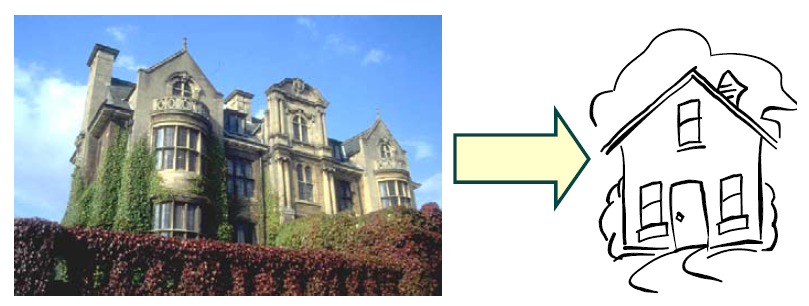
\includegraphics[width=15cm]{figure6.png}
\end{figure}

\par
(3)封装实现细节:
\par
封装填补了抽象留下的空白;抽象是指,可以让你从高层的细节,来看待一个对象;而封装则是指,除此
之外,你不能看到对象的任何其他细节层次。例如,如下图所示,封装是指,你可以从房屋的外面看,但
不能靠得太近,去将门的细节都看清楚;可以让你知道哪里有门,门是开还是关,但不能让你知道门是
木质的还是钢质的。
\begin{figure}[ht]
    \centering
    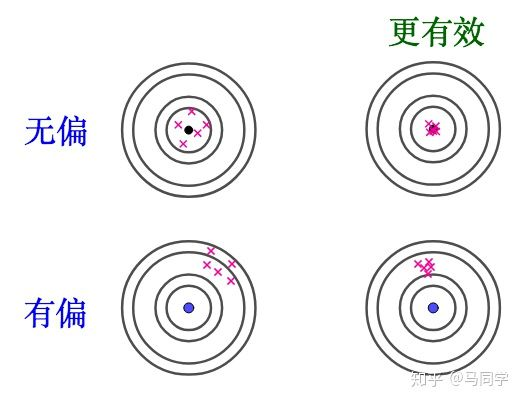
\includegraphics[width=15cm]{figure7.png}
\end{figure}

\par
(4)当继承能简化设计时就继承:
\par
在设计软件系统时,经常会发现一些大同小异的对象。例如,在一套账务系统中,包含全职员工和兼职员工,
两者的大多数数据是相同的,只是某些数据不同。在面向对象编程时,可以定义一个代表普通员工的通用类
型(general),然后把全职员工定义为普通员工,除了有一些不同之处;同样,把兼职员工也定义为普通员工,
除了一些不同之处;当一项针对员工的操作,与具体的员工类别无关时,这一操作就可以针对通用员工类型来
进行。当该操作需要区别全职员工和兼职员工时,就需要按照不同的方法来处理了。定义这种对象之间的相同点
和不同点,就叫“继承”,因为全职员工和兼职员工,都从基本员工类型继承了某些特征。
\par
继承的好处在于,它能很好地辅佐抽象的概念,并且能简化编程;因为你可以写一个基本的子程序,来处理
只依赖于门的基本属性的事项,另外写一些特定的子程序,来处理依赖特定种类门的特定操作。例如,
有些操作,如Open()或Close(),对于任何种类的门都能用,无论是防盗门还是玻璃门;编程语言如果能
支持像Open()或Close()这种,在运行期间才能确定所针对的对象的实际类型的操作,这种能力叫做
“多态”。

\par
(5)信息隐藏:
\par
信息隐藏是降低软件复杂度的一种格外重要的启发式方法,因为它强调的就是隐藏复杂度。
\begin{itemize}
    \item 隐私权:当信息被隐藏后,每个类或子程序都代表了,某种对其他类保密的设计或构建决策。
    隐藏起来的秘密,可能是某个易变的区域,或者某种文件格式,或某种数据类型的实现方式,或某个
    需要隔离的区域,在这个区域中发生的错误,不会给程序其余部分带来太大损失。在这里,类的职责
    就是把部分信息隐藏起来,并保护自己的隐私权。对系统的非重大改动,可能会影响到某个类中的
    几个子程序,但它们不应该波及到类接口的外面。
    \par
    在设计类的时候,一项关键的决策,就是确定类的哪些信息应该对外可见,而哪些信息应该隐藏起来。
    如下图所示,类的接口应该尽可能少地暴露其内部工作机制。设计类的接口与设计其他环节一样,都是
    一个迭代的过程;如果你第一次没有得到合适的接口,那么就多试几次,知道设计稳定下来;如果设计仍不
    稳定,那就需要换种方法再尝试。
    \begin{figure}[ht]
        \centering
        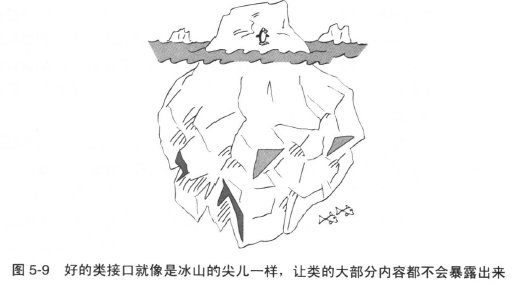
\includegraphics[width=10cm]{figure8.png}
    \end{figure}
    \item 信息隐藏的一个例子:假设你有一个程序,其中的每个对象,都是通过一个名为id的成员变量
    来保存一种唯一的ID。一种设计方法,是用一个整数来表示ID,同时用一个名为g\_maxId的全局变量,来保存
    目前已分配的ID的最大值。每当创建新的对象时,你只要在该对象的构造函数里,简单地使用
    id=++g\_maxId这条语句,就可以获得一个唯一的ID值,这种做法会让对象在创建时,执行的代码量
    最少。可这样设计可能会出错:如果你像把某些范围的ID留作它用该怎么办?如果想用非连续ID来
    提高安全性又该怎么办?如果你想重新使用已销毁对象的ID呢?如果你想增加一个断言,来确保所分配
    的ID不会超过预期的最大范围呢?如果程序中到处都是id=++g\_maxId这种语句,一旦上面说的任何
    一种情况出现,就需要修改所有这些语句。另外如果程序是多线程的,这种方法也不是线程安全的。
    \par
    创建新ID的方法就是一种你应该隐藏信息的设计决策。如果你在程序中到处使用++g\_maxId的话,就暴露
    了创建新ID的方法,即通过简单递增的方式;想法,如果你在程序中,使用语句id=NewId(),那就把创建
    新ID的方法隐藏起来了。你可以在NewId()子程序中仍然只用一行代码,return (++g\_maxId),或者
    其他与之等价的方法。如果想修改,只需修改NewId()即可。
    \par
    现假设需要把ID的类型由int改为字符串,如果在程序中大量使用了针对int的操作,例如>、<、=等等,
    这些操作并不适用字符串,那么即使改用NewId()子程序,也无济于事。因此,另一个需要隐藏的信息,就是
    ID的类型。在C++里,可以简单地使用typedef来把ID定义为IdType,也可以创建一个简单的IdType类。
    \par
    隐藏设计决策,对于减少“改动所影响的代码量”,是至关重要的。信息隐藏在设计的所有层次上,都有很大作用,
    从使用具名常量替代字面量,到创建数据类型,再到类的设计、子程序的设计以及子系统的设计等等。
    \item 两种信息:信息隐藏中所说的信息主要分为两大类,复杂度和变化源;
    \item 信息隐藏的障碍:
    \begin{itemize}
        \item 信息过度分散。例如,将100这个数字直接写到程序各个地方,会导致对它的引用过度分散;
        最好将它写入MAX\_EMPLOYEES的常量中,如果需要改动,只需要改动一处即可;
        \item 循环依赖。例如,A类中的子程序,调用了B类的中的子程序;然后B类中的子程序,又调用
        A类中的子程序;
        \item 将类内数据误认为全局数据。为了避免全局数据可能带来的问题,将类内数据误认为全局数据,
        并避免使用它。全局数据通常会受困于两类问题:一种是子程序在全局数据上执行操作,却不知道
        还有其他子程序也在用这些全局数据进行操作;另一种是子程序知道其他子程序也在用全局数据进行
        操作,但却无法明确地知道都进行了哪些操作。而类内数据就不会有这种问题,因为只有类内部的
        少数子程序才能直接访问这些数据。这些子程序不但知道有其他子程序在操纵这些数据,而且也明确
        知道具体是哪些子程序在执行这些操作。但如果设计的类包含很多体积庞大的众多子程序,那么类
        数据和全局数据之间的区别就变得模糊起来,类内数据也将开始受困于全局数据所面临的那些问题了。
        \item 可以察觉的性能损耗。如果在架构层按照信息隐藏的目标去设计系统,并不会与按照性能目标
        去设计想冲突,因此在系统架构层和编码层均避免性能上的损耗。
    \end{itemize}
    \item 信息隐藏的价值:运用了信息隐藏技术的大型项目,与没有应用这一技术的项目,修改起来大约
    容易4倍;而且信息隐藏还是结构化程序设计和面向对象设计的根基之一。
\end{itemize}

\par
(6)找出容易改变的区域:
\par
程序设计面临的最重要挑战之一,就是适应变化。需要将不稳定的区域隔离出来,从而把变化所带来的影响,
限制在一个子程序、类或包的内部。可采取的应对各种变动的措施:
\begin{itemize}
    \item 找出看起来容易变化的项目。如下是一些容易发生变化的地方:
    \begin{itemize}
        \item 业务规则:业务规则很容易成为软件频繁变化的根源。国会改变了税率结构,保险公司改变
        了它的税率表等等;如果你遵循信息隐藏的原则,那么基于这些业务规则的逻辑,就不应该遍布于整个
        程序,而是仅仅隐藏在系统的某个角落,知道需要对它进行改动,才会把它拎出来;
        \item 对硬件的依赖:与屏幕、键盘、鼠标设施以及通信设计等之间的接口,都是硬件依赖的例子。请把
        对硬件的依赖,隔离在它们自身的子系统或类中。这种隔离非常有利于把你的程序移植到新的硬件环境下。另外,
        当你为可能变化的硬件开发程序时,这样做也会有很大帮助。你可以写软件来模拟与特定硬件的交互,
        在硬件尚不稳定,或者不可用的时候,让硬件接口子系统使用该模拟器,当硬件可用的时候,把硬件接口
        子系统与模拟器切断,最终连接到真正的硬件设备上;
        \item 输入和输出:在做比纯硬件接口层稍高一些层面上的设计时,输入输出也是一个容易变化的区域。
        如果你的程序创建了自己的数据文件,那么该文件格式就可能会随软件开发的不断深化而变化。用户层
        的输入和输出格式也会变化:输出页面上字段位置、数量和排列顺序等都可能会变。因此,检查所有
        的外部接口,看看有哪些可能的变化,通常是个不错的主意;
        \item 非标准的语言特性:大多数编程语言的实现中,都包含了一些便利的、非标准的扩展。这些扩展
        可能在其他的环境中不可用;因此需要将这样的扩展单独隐藏在某个类里,以便当你转移到新的环境后,
        可以用自己写的代码区取代。与此类似,如果你使用了并非所有环境中都可用的函数库,请把这些子程序
        库隐藏在一个接口的后面,为新环境做好准备;
        \item 困难的设计区域和构建区域:将困难的设计区域和构建区域隐藏起来,也是很好的想法,因为
        这些代码可能因为设计得很差,而需要重新做;
        \item 状态变量:状态变量用于表示程序的状态,与大多数其他的数据相比,这种东西更容易改变;
        在一个典型的应用场景里,你可能一开始用布尔变量,来定义出错状态,然后又发现用具有ErrorType\_None、
        ErrorType \_Warning和ErrorType\_Fatal等值的枚举类型,来表示该状态更好。
        可以在使用状态变量时,增加至少两层的灵活性和可读性:
        \begin{itemize}
            \item 不要使用布尔变量作为状态变量,而是用枚举类型;
            \item 使用访问器子程序检查状态变量,而不是直接检测;
        \end{itemize}
        \item 隐藏数据量:例如用具名常量MAX\_EMPLOYEES来隐藏100这样的数字。
    \end{itemize}
    \item 把容易变化的项目分离出来。将容易变化的组件,单独划分成类,或者和其他容易同时发生变化的
    组件,分到同一个类中。
    \item 把容易变化的项目隔离开来。设计类之间的接口,使其对潜在的变化不敏感。
\end{itemize}
找出容易发生变化区域的一个好办法:首先找出程序中可能对用户有用的最小子集。这一子集构成了系统的
核心,不容易发生变化。接下来,用微小的步伐扩充这个系统。这里的增量可以非常微小,小到看似微不足道。
当你考虑功能上的改变时,同时也要考虑质的变化:比如让程序变成线程安全,使程序能够本地化等。这些潜在
的改进区域,就构成了系统中的潜在变化。请依照信息隐藏的原则,来设计这些区域。通过首先定义清楚核心,
你可以认清哪些组件属于附加功能,这是就可以把它们提取出来,并把它们的可能改进隐藏起来。

\par
(7)保持松散耦合:
\par
耦合度表示类与类之间,或子程序与子程序之间的关系紧密程度。耦合度设计的目标,是创建出小的、直接的、
清晰的类或子程序,使它们与其他类或子程序之间,关系尽可能地灵活,这就被称作“松散耦合”。模块之间
良好的耦合关系,需要松散到恰好能使一个模块,能够很容易地被其他模块使用,确保模块之间的连接关系
尽可能的简单。尽量使创建的模块,不依赖或很少依赖其他模块。例如sin()这样的子程序是松耦合的,因为它
需要知道的东西,也就是一个传入的、代表角度的数值。而像InitVars(var1,...,varN)这样的子程序,则耦合
得过于紧密,因为在调用端,必须传入各个参数,调用它的模块实际上知道在InitVars()内部会做些什么。
如果两个类都依赖于同一个全局变量的使用,那么它们之间的耦合关系就更紧密了。
\begin{itemize}
    \item 耦合标准:下面是一些在衡量模块之间耦合度使,可采用的标准
    \begin{itemize}
        \item 规模。指模块之间的连接数。只有1个参数的子程序,相比有6个参数
        的子程序,耦合度更高;
        \item 可见性。指两个模块之间,连接的显著程度。在程序开发过程中,需要把模块之间的连接关系,
        变得广为人知而获取信任。通过参数表传递数据,则是一种明显连接,值得提倡;而通过修改全局数据,
        进而使另一个模块能使用该数据,则是一种不好的设计;
        \item 灵活性。指模块之间的连接,是否容易改动。一个模块越容易被其他模块调用,那么它们之间
        的耦合关系,就会越松散,并且更易于维护。因此,在创建系统架构时,应按照“尽可能缩减相互连接”的
        准则,来分解程序。
    \end{itemize}
    \item 耦合种类:几种常见的几种耦合,
    \begin{itemize}
        \item 简单数据类型的参数耦合。当两个模块之间,通过参数来传递数据,并且所有的数据都是简单
        数据类型时,这两个模块之间的耦合关系,就是简单数据参数耦合的。这种耦合关系是正常且可以接受的。
        \item 简单对象耦合。如果一个模块实例化一个对象,那么它们之间的耦合关系,就是简单对象耦合的。
        这种耦合关系也很不错。
        \item 对象参数耦合。如果Object1要求Object2传给它一个Object3,那么这两个模块就是对象参数耦合的。
        与Object1仅要求Object2传递给他简单数据类型相比,这种耦合关系要更紧密些,因为它要求Object2
        了解Object3。
        \item 语义上的耦合。最难缠的耦合关系是这样发生的:一个模块不仅使用了另一个模块的语法元素,
        而且还使用了有关那个模块内部工作细节的语义知识。例如Module1向Module2传递了一个控制标志,
        用它告诉Module2该做什么,这种方法要求Module1对Module2的内部工作细节有所了解,也就是说需要
        了解Module2对控制标志的使用。语义上的耦合是非常危险的,因为更改被调用模块中的代码,可能会
        破坏调用它的模块,破坏的方式是编译器完全无法检查的。类似这样的代码崩溃时,其方式是非常微妙的,
        看起来与被使用的模块中的代码更改毫无关系,因此会使得调试工作变得无比困难。
    \end{itemize}
\end{itemize}
\par
松散耦合的关键之处在于,一个有效的模块提供了一层附加的抽象:一旦你写好了它,就可以想当然地去用它。
这样就降低了整体系统的复杂度,使得你可以在同一时间,只关注一件事。如果对一个模块的使用,要求你
同时关注好几件事:其内部工作的细节、对全局数据的修改、不确定的功能点等;那么就失去了抽象的能力,
模块所具有的管理复杂度的能力也就削弱或完全丧失了。

\par
(8)查阅常用的设计模式:
\par
设计模式精炼了众多现成的解决方案,可以解决很多软件开发中,最常见的问题。有些软件问题要求
全新的解决方案,但是大多数问题都和过去遇到的问题类似,因此可以使用类似的解决方案或者模式加以解决。
下表为常见的设计模式:
\begin{figure}[ht]
    \centering
    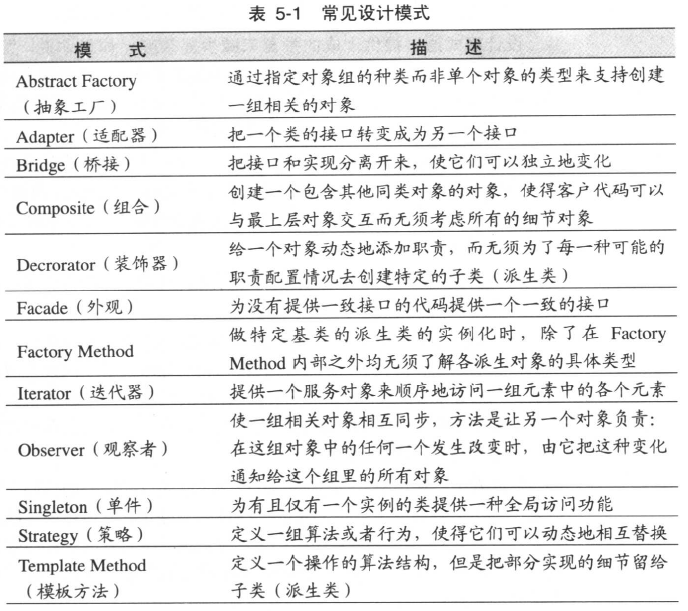
\includegraphics[width=10cm]{figure9.png}
\end{figure}
\par
与完全定制的设计方案相比,设计模式提供了下列好处:
\begin{itemize}
    \item 设计模式通过提供现成的抽象,来减少复杂度;
    \item 设计模式通过把常见解决方案的细节,通过制度化来减少出错;
    \item 设计模式通过提供多种设计方案,带来启发性的价值;
    \item 设计模式通过把设计对话,提升到一个更高的层次上,来简化交流。
\end{itemize}
\par
应用设计模式的一个潜在陷阱,是强迫让代码适用于某个模式。有时候,对代码进行一些微小的更改,
以便符合某个广为人知的模式,会使这段代码更容易理解。但是,如果一段代码做出巨大改动,迫使它
去符合某个标准设计模式,有时反而会把问题复杂化。

\par
(9)使用启发式方式的原则:
\par
最有效的原则之一,就是不要卡在单一的方法上。如果用UML画设计图不可行,那么就直接用英语写;
写段简短的测试程序;尝试一种截然不同的方法;用铅笔画出轮廓和草图来指导思维等等。
\par
你无须马上解决整个设计难题。一旦被卡住了,那么请记住回过头来时,有一处地方需要做决策,但眼下
你还没有足够的信息来解决这个问题。如果你尝试了一些设计方案,但没有很好的解决问题的时候,更自然
的方式,是让那些问题留在未解决的状态,等拥有更多信息后,在去做。

\subsection{设计实践}
在设计过程中,可以采用如下一些工作步骤,以便获得良好的设计结果:
\par
(1)迭代
\par
设计是一个迭代的过程。当在备选的方案之中,循环并尝试一些不同的做法时,将会同时从高层和低层的不同
视角,去审视问题。从高层视角从得到的大范围图景,有助于你把相关的低层细节纳入考虑;从低层视角中
获得的细节,也会为你的高层决策奠定基础。这种高低层面之间的互动,被认为是一种良性的原动力,它
所创建的结构,要远远稳定于单纯自上而下,或自下而上创建的结构。

\par
(2)分而治之
\par
没有人的头脑能装下一个复杂程序的全部细节,对设计同样适用。将程序分解为不同的关注区域,然后
分别处理每一个区域;如果在某个区域里碰上了死胡同,那么就迭代。

\par
(3)自上而下和自下而上
\begin{itemize}
    \item 自上而下的设计:是指从某个很高的抽象层次开始,定义出基类或其他不那么特殊的设计元素;在开发
    这一设计的过程中,逐渐增加细节的层次,找出派生类、合作类,以及其他更细节的设计元素。
    这种设计方式可以看作是一层层分解的过程,在分解过程的不同阶段,需要选择用什么方法,去分解
    子系统,给出继承关系树,形成对象的组合。持续分解,直到在下一层,直接编码比分解更容易。
    \item 自下而上的设计:是指设计始于细节,向一般性延伸;这种设计通常是从寻找具体对象开始,最后从细节之中生成
    对象以及基类。需要考虑的一些步骤:
    \begin{itemize}
        \item 对系统需要做的事项,有哪些已知条件;
        \item 找出具体的对象和职责;
        \item 找出通用的对象,把它们按照适当方式组织起来:子系统、包、对象组合,或者继承;看哪种方式合适;
        \item 在更上一层继续设计,或者回到最上层,尝试向下设计
    \end{itemize}
    \item 两者并不矛盾:两种策略最关键的区别在于,自上而下是一种分解策略;而自下而上是一种合成策略;
    前者从一般性的问题出发,把该问题分解成可控的部分;后者从可控的部分出发,去构造一个通用的方法。
\end{itemize}

\par
(4)建立试验性原型
\par
有些时候,除非能很好的了解实现细节,否则很难判断一种设计方法是否凑效。例如,在知道它能满足性能要求
之前,很难判断某种数据库的组织结构是否适用。此时,建立试验性原型,便能低成本解决这些问题:写出用于
回答特定设计问题的、量少且能够随时扔掉的代码。但是使用试验原型,存在以下一些风险:
\begin{itemize}
    \item 开发人员没有遵循“用最少代码回答提问”的原则。例如,设计问题是“我们选的的数据库框架,
    能否支撑所需的交易量?”,你不需要为了这一问题,而编写任何产品代码,也不需要去了解数据库的详情;
    只需要了解能估计出问题范围的最少信息:有多少张表、表中有多少条记录等等,接下来就可以用Table1、
    Table2、Column1、Column2等名字,写出最简单的原型代码,往表里随意填入些数据,然后做你所
    需要的性能测试;
    \item 设计的问题不够特殊。例如,设计问题“这样的数据库框架,能否工作?”,并没有为建立原型提供多少
    指引;而像“这个数据库框架能不能在X、Y和Z的前提下,支持每秒1000次交易?”这样的问题,则能
    为建立原型,提供更坚实的基础;
    \item 开发人员不把原型代码当作可抛弃的代码。如果开发人员相信某段代码,将被用在最终产品里,
    那么他根本不可能写出最少数量的代码来。避免产生这一问题的一种做法,是用与产品代码不同的技术,
    来开发原型。例如用Python来为C++设计做原型。
\end{itemize}


\par
(5)合作设计
\par
无论组织形式的正式与否,在设计过程中,三个臭皮匠顶得上一个诸葛亮,合作可以以任意方式展开。例如,
随便走到一名同事办公桌前,向他征求一些想法;结对编程等等。


\par
(6)做多少设计才足够
\par
对于实施正式编码前的设计工作量和设计文档的正规程度,很难有个确定的定论,下表可以做个参考,
\begin{figure}[ht]
    \centering
    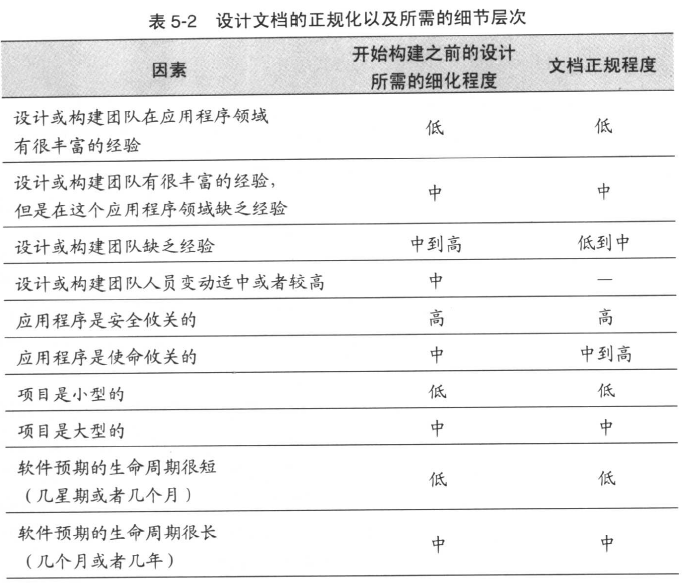
\includegraphics[width=10cm]{figure10.png}
\end{figure}
\par
如果在编码前,还没法判断是否应该做更多深入设计,那么宁愿去做更详细的设计。最大的设计失误,来自于
误认为自己已经做得很充分,可事后却发现还是做得不够。另一方面,也不要太过于专注,对设计进行文档化,
而导致失败;程序化的活动,容易把非程序化的活动驱逐出去,过早地去润色设计方案,就是所描述的例子。

\par
(7)记录设计成果
\par
传统的记录设计成果的方式,是把它写成正式的设计文档;然而,你还可以用很多种方法来记录设计成果,
这些方法对于那些小型的、非正式项目,或者只需要轻量级地记录设计成果的项目,效果是很不错的:
\begin{itemize}
    \item 把设计文档插入到代码里:在代码注释中写明关键的设计决策,通常放在文件或类的开始位置;
    \item 用Wiki来记录设计讨论和决策;
    \item 写总结邮件;
    \item 使用数码相机;
    \item 保留设计挂图;
    \item 使用CRC卡片(类、职责、合作者);
    \item 在适当的细节层,创建UML图。
\end{itemize}


\section{可以工作的类}
类是由一组数据和子程序构成的集合,这些数据和子程序共同拥有一组内聚的、明确定义的职责。类也可以
只是由一组子程序构成的集合,这些子程序提供一组内聚的服务,哪怕其中未涉及共用的数据。成为高效
程序员的一个关键,在于当你开发程序任一部分的代码时,都能安全地忽视程序中尽可能多的其余部分。
而类就是实现这一目标的首要工具。

\subsection{类的基础:抽象数据类型}
抽象数据类型(ADT,abstract data type)是指一些数据,以及对这些数据所进行的操作的集合。这些操作,
既是像程序的其余部分描述了这些数据是怎么样的,也允许程序的其余部分改变这些数据。一个ADT可能是一个图形
窗体,以及所有能影响该窗体的操作;也可以是一个文件,以及对这个文件进行的操作等等。
\par
(1)一个ADT例子:
\par
假如你正在写一个程序,控制文本的字体,它能用不用的字型、字号等;如果用一个ADT,就能在相关数据上,
捆绑一组操作字体的子程序;相关的数据包括字体名称、字号和文字属性等。这些子程序和数据集合,就是
一个ADT。
\par
如果不使用ADT,就只能用一种拼凑的方法来操纵字体了。例如,如果要将字体大小改为12磅(point),
即高度为16像素(pixel),那么就需要这样的代码:
\par
currentFont.sizeOnPixels = PointsToPixels(12)
\par
\noindent 但不能同时使用currentFont.sizeInPixels和currentFont.sizeInPoints;因为如果你同时使用
这两项数据成员,currentFont就无从判断到底该用哪个。而且,如果你在程序很多地方都需要修改字体
大小,那么这类语句就会散步在整个程序中。如果需要把字体设为粗体,或许需要写成这样:
\par
currentFont.attribute = CurrentFont.attribute or 0x02 或
\par
currentFont.bold = True
\par
\noindent 这些做法都存在一个限制,即要求调用方代码,直接控制数据成员,这无疑限制了currentFont的使用。

\par
(2)使用ADT的好处
\par
\begin{itemize}
    \item 可以隐藏实现细节:把信息隐藏起来,能保护程序的其余部分不受影响。
    \item 改动不会影响到整个程序:如果数据类型改变,只需在一处修改而不会影响到整个程序。
    \item 让接口能提供更多信息:把所有相似的操作,都集中到一个ADT中,就可以基于磅数或像素
    来定义整个接口,或者把二者明确区分开,从而有助于避免混淆。
    \item 更容易提高性能:如果想提高操作字体时的性能,就可以重新编写出一些更好的子程序,
    而不用来回修改整个程序。
    \item 让程序的正确性更显而易见:验证像currentFont.attribute = CurrentFont.attribute or 0x02
    的语句是否正确,是很枯燥的,可以替换成像currentFont.SetBoldOn()这样的语句,验证它
    是否正确就更容易一些。
    \item 程序更具自我说明性:可以改进currentFont.attribute = CurrentFont.attribute or 0x02
    这样的语句:将0x02换成BOLD,但无论怎么杨修,其可读性都不如currentFont.SetBoldOn()
    这条语句。
    \item 无须在程序内到处传递数据:在上面的例子中,必须直接修改currentFont的值,或把它传给
    每一个要操作字体的子程序;如果使用了ADT,就不用再在程序里到处传递currentFont了。
    \item 可以像在现实世界中那样操作实体,而不用在底层实现上操作它:可以定义一些针对字体
    的操作,这样程序的绝大部分,就能完全以“真实世界中的字体”这个概念来操作,而不再用数组访问、结构体
    定义、True与False等这些底层的实现概念了。
\end{itemize}
为了定义一个ADT,只需要定义一些用来控制字体的子程序,例如:
\par
currentFont.SetSizeInPoints(sizeInPoints)
\par
currentFont.SetSizeInPixels(sizeInPixels)
\par
currentFont.SetBoldOn()
\par
currentFont.SetBoldOff()

\par
(3)使用ADT的一些建议:
\par
\begin{itemize}
    \item 把常见的底层数据类型构建为ADT,并使用这些ADT,而不再使用底层数据类型:堆栈、列表、
    队列,以及几乎所有常见的底层数据类型,都可以用ADT表示;如果堆栈代表的是一组员工,就该把它
    看作是一些员工,而不是堆栈;如果列表代表一个出场演员名单,就该把它看作是出场演员名单,而不是列表等等。
    \item 把像文件这样的常用对象当成ADT。
    \item 简单的事物也可当作ADT:例如,一盏灯只有开和关两种操作,也可以放到ADT里,这样可以
    提高代码的自我说明能力,并减少需要到处传递的数据。
    \item 不要让ADT依赖于存储介质:假设有一张保险费率表,它太大了,因此只能保存在磁盘上;
    你可能编写出rateFile.Read()这样的访问器子程序,然而当你把它当作一个“文件”时,就已经暴露
    了过多的数据信息,一旦对程序进行修改,把这张表存到内存中,而不是磁盘上,把它当作文件的
    那些代码将不正确,而且产生误导并使人迷惑。因此,请尽量让类和访问器子程序的名字,与存储数据的方式
    无关,并只提及抽象数据类型本身,例如rateTable.Read()或更简单rates.Read()。
\end{itemize}

\subsection{良好的类接口}
创建高质量的类,第一步,可能也是最重要的一步,就是创建好的接口。这也包括了创建一个可以通过接口来
展现的合理抽象,并确保细节仍被隐藏在抽象背后。
\par
(1)好的抽象:
\par
抽象是一种以简化的形式,来看待复杂操作的能力。类的接口为隐藏在其后的具体实现,提供了一种抽象。
类的接口应能提供一组明显相关的子程序。
\par
假设有一个实现雇员(Employee)这一实体的类,其中可能包含雇员的姓名、地址、电话号码等数据,以及一些用
来初始化并使用雇员的服务子程序,例如:
\begin{lstlisting}
    C++示例:展现良好抽象的类接口
    class Employee {
    public:
        // public constructors and destructors
        Employee();
        Employee(
            FullName name,
            String address,
            String workPhone,
            String homePhone,
            TaxId taxIdNumber,
            JobClassification jobClass
        );
        virtual ~Employee();
        // public routines
        FullName GetName() const;
        String GetAddress() const;
        String GetWorkPhone() const;
        String GetHomePhone() const;
        TaxId GetTaxIdNumber() const;
        JobClassification GetJobClassification() const;
        ...
    private:
        ...
    };
\end{lstlisting}
在类的内部,还可能会有支持这些服务的其他子程序和数据,但类的使用者,并不需要了解它们;类接口的
抽象能力非常有价值,因为接口中的每个子程序,都在朝这个一致的目标而工作。
\par
一个没有经过良好抽象的类,可能会包含有大量混杂的函数,例如
\begin{lstlisting}
    C++示例:展现不良抽象的类接口
    class Program {
    public:
        ...
        //public routines
        void InitializeCommandStack();
        void PushCommand( Command command );
        Command PopCommand();
        void ShutdownCommandStack();
        void InitializeReportFormatting();
        void FormatReport( Report report );
        void PrintReport( Report report );
        void InitializaeGlobalData();
        void ShutdownGlobalData();
        ...
    private:
        ...
    };
\end{lstlisting}
其中有很多子程序,有用来操作命令栈的,有用来格式化报表的,有用来打印报表的,还有用来初始化全局数据的。
在命令栈、报表和全局数据之间,很难看出什么联系。类的接口不能展现出一种一致的抽象,因此它的
内聚性就很弱;应该把这些子程序,重新组织到几个职能更专一的类里去,在这些类的接口中,提供更好的
抽象。
\par
如果这些子程序是一个叫做Program类的一部分,那么可以这样来修改它,以提供一种一致的抽象:
\begin{lstlisting}
    C++示例:能更好展现抽象的类接口
    class Program{
    public:
        ...
        // public routines
        void InitializeUserInterface();
        void ShutdownUserInterface();
        void InitializeReports();
        void ShubtdownReports();
        ...
    private:
        ...
    };
\end{lstlisting}
在清理这一接口时,将原有的一些子程序,转移到其他更适合的类里面,而把另一些转为InitializeUserInterface()
和其他子程序中使用的私有子程序。
\par
这种对类的抽象进行评估的方法,是基于类所具有的public子程序所构成的集合,即类的接口。即使类的
整体表现出一种良好的抽象,类内部的子程序也未必都能表现出良好的抽象,也同样要把它们设计得可以表现出
很好的抽象。
\par
一些创建类的抽象接口的指导建议:
\begin{itemize}
    \item 类的接口应该展现一致的抽象层次:在设计类的时候,有一种很好的方法,就是把类看作一种
    用来实现ADT的机制;每一个类应该实现一个ADT,并且仅实现这一个ADT。如果你返现某个类实现了不止
    一个ADT,或者你不能确定究竟它实现了何种ADT,你就应该把这个类,重新组织为一个或多个定义
    更加明确的ADT。
    \begin{lstlisting}
        C++示例:混合了不同层次抽象的类接口
        class EmployeeCensus: public ListContainer {
        public:
            ...
            // public routines
            void AddEmployee( Employee employee );
            void RemoveEmployee( Employee employee );

            Employee NextItemInList();
            Employee FirstItem();
            Employee LastItem();
            ...
        private:
            ...
        };
    \end{lstlisting}
    这个类展现了两个ADT:Employee和ListContainer。出现这种混合的抽象,通常是源于程序员使用容器类
    或其他类库来实现内部逻辑,但却没有把“使用类库”这一事实隐藏起来。下面是隐藏了实现细节的类接口:
    \begin{lstlisting}
        class EmployeeCensus {
        public:
            ...
            // public routines
            void AddEmployee( Employee employee );
            void RemoveEmployee( Employee employee );
            Employee NextEmployee();
            Employee FirstEmployee();
            Employee LastEmployee();
            ...
        private:
            ListContainer m_EmployeeList;
            ...
        };
    \end{lstlisting}
    \item 一定要理解类所实现的抽线是什么:一些类非常像,必须非常仔细地理解类的接口,应该捕捉的
    抽象到底是哪一个。当你不得不在两个相似的抽象之间做出选择时,请确保你的选择是正确的。
    \item 提供成对的服务:大多数操作都有和其相应的、相等的以及相反的操作。如果有一个操作用来把
    灯打开,那很有可能也需要另一个操作,来把灯关闭。在设计类的时候,需要检查每一个public子程序,
    决定是否需要另一个与其互补的操作。不要盲目地创建相反操作,但你一定要考虑,看看是否需要它。
    \item 把不相关的信息转移到其他类中:有时你会发现,某个类中,一般子程序使用着该类的一半数据,
    而另一半子程序则使用另一半数据。这时你其实已经把两个类混在一起使用了,这就需要把它们拆开。
    \item 尽可能让接口可编程,而不是表达语义:每个接口都由一个可编程的部分和一个语义部分组成。
    可编程的部分,由接口中的数据类型和其他属性构成,编译器在检查编译错误时,能强制性地要求它们。
    而语义部分则由“本接口将会被怎样使用”的假定组成,而这些是无法通过编译器来强制实施的。例如,
    语义接口中包含的考虑“RoutineA必须在RoutineB之前被调用”。语义接口应通过注释说明,但要尽可能
    让接口不依赖于这些说明。一个接口中任何无法通过编译器强制实施的部分,就是一个可能被误用的
    部分。要想办法把语义接口的元素,转换为编程接口的元素,比如用断言或其他的技术。
    \item 谨防在修改时破坏接口的抽象:在对类进行修改和扩展的过程中,常常会发现额外所需的一些功能;
    这些功能并不十分适应于原有的类接口,可看上去却很难用另一种方法实现。例如,上面的Employee类
    演变成了下面这个样子:
    \begin{lstlisting}
        C++语言示例:在维护时被破坏的类接口
        class Employee {
        public:
            ...
            // public routines
            FullName GetName() const;
            Address GetAddress() const;
            PhoneNumber GetWorkPhone() const;
            ...
            bool IsJobClassificationValid( JobClassification jobClass );
            bool IsZipCodeValid( Address address );
            bool IsPhoneNumberValid( PhoneNumber phoneNumber );
            SqlQuery GetQueryToCreatNewEmployee() const;
            SqlQuery GetQueryToModifyEmployee() const;
            SqlQuery GetQUeryToRetrieveEmployee() const;
            ... 
        private:
            ...
        };
    \end{lstlisting}
    前面代码示例中的清晰抽线,现在已经变成了,由一些零散功能组成的大杂烩。在雇员和检查邮政
    编码、电话号码或职位的子程序之间,并不存在什么逻辑上的关联,那些暴露SQL语句查询细节的子程序,
    所处的抽象层次比Employee类也要低得多,它们都破坏了Employee类的抽象。
    \item 不要添加与接口抽象不一致的公用成员:每次你向类的接口中,添加子程序时,问问“这个子程序
    与现有接口所提供的抽象一致吗”,如果发现不一致,就要换另一种方法来进行修改,以便能保持抽象的
    完整性。
    \item 同时考虑抽象性和内聚性:抽象性和内聚性这两个概念之间的关系,非常紧密:一个呈现出很好
    的抽象的类接口,通常也有很高的内聚性。而具有很强内聚性的类,往往也会呈现为很好的抽象。关注类的
    接口所表现出来的抽象,比关注类的内聚性更有助于深入地理解类的设计。如果你发现某个类的内聚性很弱,
    也不知道该怎么改,那就换一种方法,问问你自己这个类是否表现为一致的抽象。
\end{itemize}

\par
(2)良好的封装
\par
封装是一个比抽象更强的概念。抽象通过提供一个,可以让你忽略实现细节的模型,来管理复杂度;而封装则
强制阻止你看到细节,即便你想这么做。这两个概念之所以相关,是因为没有封装时,抽象往往很容易被打破。
依据经验,要么就是封装与抽象两者皆有,要么就是两者皆失。除此之外,没有其他可能。
\begin{itemize}
    \item 尽可能地限制类和成员的可访问性:让可访问性尽可能低,是促成封装的原则之一。当你在犹豫
    某个子程序的可访问性,应该设为public、private还是protected时,经验之举应该采用最严格且可行的
    访问级别。这是一个很好的指导建议,但还有更重要的建议,即考虑“采用哪种方式,最好地保护接口抽象
    的完整性?”,如果暴露一个子程序不会让抽象变得不一致的话,这么做就很可能是可行的。如果不
    确定,那么多隐藏,通常比少隐藏要好。
    \item 不要公开暴露成员数据:暴露成员数据会破坏封装性,从而限制你对这个抽象的控制能力。例如,一个Point
    类如果暴露了下面这些成员的话:
    \begin{lstlisting}
        float x;
        float y;
        float z;
    \end{lstlisting}
    它就破坏了封装性,因为调用该类可以自由地使用Point类里面的数据,而Point类却连这些数据什么
    时候被改动过都不知道。然而,如果Point类暴露的是这些方法的话:
    \begin{lstlisting}
        float GetX();
        float GetY();
        float GetZ();
        void SetX(float x);
        void SetY(float y);
        void SetZ(float z);
    \end{lstlisting}
    那它还是封装完好的。你无法得知底层实现用的是不是float x、y、z,也不会知道Point是不是把这些
    数据保存为double然后再转换成float,也不可能知道Point是不是把它们保存在月亮上,然后再从
    外层空间中的卫星上把它们找回来。
    \item 避免把私有的实现细节放入到类的接口中:做到真正的封装后,程序员们是根本看不到任何实现细节的。
    无论是在字面上还是在喻意,它们都被隐藏了起来。然而,包括C++在内的一些流行编程语言,却从结构上,
    要求程序员在类的接口中透露实现细节。例如,
    \begin{lstlisting}
        C++示例:暴露类内部实现细节
        class Employee {
        public:
            ...
            Employee{
                FullName name,
                String address,
                String workPlace,
                String homePhone,
                TaxId taxIdNumber,
                JobClassification jobClass
            };
            ...
            FullName GetName() const;
            String GetAddress() const;
            ...
        private:
            String m_Name;
            String m_Address;
            int m_jobClass;
            ...
        };
    \end{lstlisting}
    其中,private中的私有成员变量,暴露了实现细节。将private段的声明放在类的头文件中,看上去
    似乎只是小小地违背了原则,但它实际上是在鼓励程序员们查阅实现细节。在这个例子中,客户代码本意是
    要使用Address类型来表示地址信息,但头文件中却把“地址信息用String来保存”,这一实现细节暴露了出来。
    为解决这一问题,建议将类地接口与类的实现隔离开,并在类的声明中包含一个指针,让该指针指向类的实现,
    但不能包含任何其他实现细节。
    \begin{lstlisting}
        C++示例:隐藏类的实现细节
        class Employee {
        public:
            ...
            Employee( ... );
            ...
            FullName GetName() const;
            String GetAddress() const;
            ...
        private:
            EmployeeImplementation *m_implementation;
        }
    \end{lstlisting}
    现在你就可以把实现细节,放到EmployeeImplementation类里了,这个类只对Employee类可见,而对使用
    Employee类的代码来说,则是不可见的。
    \item 不要对类的使用者做任何假设:类的设计和实现,应该符合类的接口中所隐含的契约。它不应该对接口
    会被如何使用,或不会被如何使用,做出任何假设;除非在接口中有明确说明。例如下面这样一段注释,就显示
    出这个类,过多地假定了它的使用者:
    \begin{lstlisting}
        请将x、y和z初始化为1.0,因为如果把它们
        初始化为0.0,DerivedClass就会崩溃。
    \end{lstlisting}
    \item 避免使用友元类(friend class):友元类会破坏封装,因为它让你在同一时刻,需要考虑更多的代码
    量,从而增加了复杂度。
    \item 不要因为一个子程序里,仅使用公用子程序,就把它归入到公开接口。
    \item 让阅读代码比编写代码更方便:为了让编写代码更方便,而降低代码的可读性,是非常不经济的。尤其
    是在创建类的接口时,即使某个子程序与接口的抽象不是很相配,有时人们也往往把这个子程序加到接口里,
    从而让正开发的这个类的某处调用代码,能更方便地使用它。然而,这段子程序的添加,正时代码走下坡路的开始。
    \item 要格外警惕从语义上破坏封装性:比较起来,语义上的封装和语法上的封装,二者的难度相差无几。从语法
    的角度说,要想避免窥探另一个类的内部实现细节,只要把它内部的子程序和数据,都声明为private就可以了,
    这是相对容易办到的。然而,要想达到语义上的封装,就完全时另一回事了。下面一些类的调用方代码例子,从
    语义上破坏了其封装性:
    \begin{itemize}
        \item 不去调用A类的InitializeOperations()子程序,因为你知道A类的PerformFirstOperation()
        子程序会自动调用它。
        \item 不在调用employee.Retrivae(database)之前调用database.Connect()子程序,因为你知道在未建立
        数据库连接的时候,employee.Retrieve()会去连接数据库的。
        \item 不去调用A类的Terminate()子程序,因为你知道A类的PerformFinalOperation()子程序已经调用它了。
        \item 即便在ObjectA离开作用域之后,你仍然去使用由ObjectA创建的、指向ObjectB的指针或引用,因为
        你知道ObjectA把ObjectB放置在静态存储空间中了,因此ObjectB肯定还可以用。
        \item 使用ClassB.MAXIMUM\_ELEMENTS而不用ClassA.MAXIMUM\_ELEMENTS,因为你知道它们两个的值是
        相等的。
    \end{itemize}
    上面这些例子的问题都在于,它们让调用方代码不是依赖类的公开接口,而是依赖类的私用实现。每当你发现自己
    是通过查看类的内部实现,来得知如何使用这个类的时候,你就不是在针对接口编程了,而是透过接口针对
    内部实现编程了。如果你透过接口来编程的话,封装性就被破坏了,而一旦封装性开始遭到破坏,抽象能力就快遭殃了。
    如果仅仅根据类的接口文档,还是无法得知如何使用一个类的话,正确的做法不是拉出这个类的源代码,从中
    查看其内部实现,而是应该联系类的作者,告诉他“我不知道该怎么用这个类”。而对于类的作者来说,正确的
    做法,不是面对面地告诉你答案,而是从代码库中check out类地接口文件,修改类地接口文档,再把文件check in
    回去,然后告诉你“看看现在你知不知道该怎么用它了”。
    \item 留意过于紧密的耦合关系:耦合是指两个类之间关联的紧密程度。通常这种关联越松越好。一些建议:
    \begin{itemize}
        \item 尽可能地限制类和成员地可访问性。
        \item 避免友元类,因为它们之间是紧密耦合地。
        \item 在基类中把数据声明为private,而不是protected,以降低派生类和基类之间耦合地程度。
        \item 避免在类地公开接口中,暴露成员数据。
        \item 要对从语义上破坏封装性保持警惕。
        \item 察觉“Demeter法则”。
    \end{itemize}
    耦合性与抽象和封装性,有着非常紧密的联系。紧密的耦合性,总是发生在抽象不严谨,或封装性遭到破坏的时候。
    如果一个类提供了一套不完整的服务,其他的子程序就可能要去直接读写该类的内部数据。这样一来,就把类给拆开了,
    把它从一个黑盒子,变成了一个玻璃盒子,从而事实上消除了类的封装性。
\end{itemize}

\subsection{有关设计和实现问题}
给类定义合理的接口,对于创建高质量程序,起到了关键作用。然而,类内部的设计和实现也同样重要。这一节
就来论述关于包含、继承、成员函数和数据成员、类之间的耦合性、构造函数、值对象与引用对象等问题。
\par
(1)包含:“有一个...”的关系
\par
包含是一个非常简单的概念,它表示一个类含有一个基本数据元素或对象。
\begin{itemize}
    \item 通过包含实现“有一个”的关系:例如,一名雇员“有一个”姓名、“有一个”电话号码等,通常,你可以让姓名、
    电话号码成为Employee类的数据成员,从而建立这种关系。
    \item 在万不得已时通过private继承来实现“有一个”的关系:在某些情况下,你会发现根本无法,使用将一个
    对象当作另一个对象的成员的办法,来实现包含关系。一些专家建议,此时可采用private继承所要包含的对象
    的办法。这么做的主要原因,是要让外层的包含类,能够访问内层被包含类的protected成员函数与数据成员。
    然而在实践中,这种做法会在派生类与基类之间,形成一种过于紧密的关系,从而破坏了封装性。而且,这种做法
    也往往会带来一些设计上的错误,而这些错误是可以用“private继承”之外的其他方法解决的。
    \item 警惕有超过约7个数据成员的类:研究表明,人们在做其他事情时,能记住的离散项目的个数是7±2。
    如果一个类包含有超过约7个数据成员,请考虑要不要把它分解为几个更小的类。如果数据成员都是整型或
    字符串这种简单数据类型,可以按7±2的上限考虑;反正,如果数据成员都是复杂对象的话,就应按7±2的下限
    来考虑了。
\end{itemize}
\par
(2)继承:“是一个...”的关系
\par
继承的概念是说一个类是另一个类的一种特化。继承的目的在于,通过“定义能为两个或更多个派生类提供共有元素的
基类”的方式,写出更精简的代码。其中共有元素可以是子程序接口、内部实现、数据成员或数据类型等。继承
能把这些共有的元素集中在一个基类中,从而有助于避免在多处出现重复的代码和数据。


\subsection{创建类的原因}

\subsection{超越类:包}

\section{高质量的子程序}

\section{防御式编程}

\section{伪代码编程过程}

\section{使用变量的一般事项}

\section{变量名的力量}


\section{基本数据类型}

\section{不常见的数据类型}

\section{组织直线型代码}

\section{条件语句}

\section{控制循环}

\section{不常见的控制结构}

\section{表驱动法}

\section{一般控制问题}

\section{软件质量概述}

\section{协同构建}

\section{开发者测试}

\section{调试}

\section{重构}

\section{代码调整策略}

\section{代码调整技术}

\section{程序规模对构建的影响}

\section{管理构建}

\section{集成}

\section{编程工具}

\section{布局与风格}

\section{自说明代码}

\section{个人性格}

\section{软件工艺}

\section{更多信息}


\begin{thebibliography}{99}  
    \bibitem{Meyer2000}Meyer CD (2000) Matrix Analysis and Applied Linear Algebra. Philadelphia, PA: SIAM.
    \bibitem{consistency} Agostino Martinelli. Closed-form solution of visual-inertial structure from motion. International
    Journal of Computer Vision, Springer Verlag, 2013. ￿hal-00905881
\end{thebibliography}



\end{document}

